\chapter{Event Selection}
\label{event_selection_chapter}

In this chapter we discuss the acceptance region for this analysis, as well as
how events are selected both by the detector and for the analysis. Additionally
we discuss the background that makes it through the selection process.

\section{Acceptance}
\label{sec:acceptance}

The acceptance region is a definition of what events, assuming that there are
no limitations due to the detector design, are include in the analysis. The
acceptance region is what the final result of this analysis will be corrected
to, ensuring that other measurements and theoretical predictions can be
compared to our results without having to account for the detector response.
The acceptance region defines what sort of physics results we can make
statements about, and also determines the value of the effective cross-section
of the \Z.

Our acceptance is defined by the kinematics of the two electrons and the mass
of the Z boson. One of the electrons, called the \CentralElectron, is required
to have $\pt > 30 \GeV$ and to be within the central region of the detector
(hence the name) with $|\eta| < 2.1$. The other electron, called the
\ExtendedElectron, has looser requirements; it must have $\pt > 20 \GeV$ and is
not required to be as central with $|\eta| < 2.4$. The requirements on the
\CentralElectron were selected in conjunction with the \Ztomumu measurement of
\phistar at CMS so that that measurement and this one could be easily combined
into a joint measurement. The pseudorapidity limit was selected to match the
most efficient region of CMS's single muon trigger, while the transverse
momentum threshold was dictated by threshold on single electron trigger. The
pseudorapidity limit on the \ExtendedElectron was chosen to keep all of the
electrons within the region covered by the tracker (which allows a better
angular measurement than ECAL alone), while the transverse momentum threshold
was selected because for $\pt < 20 \GeV$ the rate of fake electrons increases.

\begin{figure}[!htbp]
    \centering
    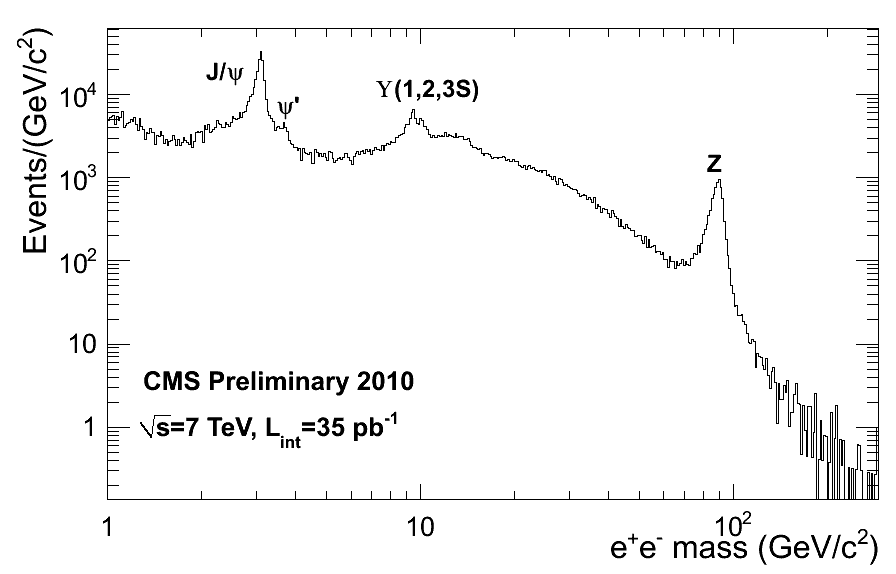
\includegraphics[width=\textwidth]{figures/dielectron_mass_7tev.png}
    \caption{The spectrum of \ee events as measured by CMS in 2010.}
    \label{fig:ee_spectrum}
\end{figure}

There are other particles, like the \jpsi, that decay to \ee pairs as shown in
\FIG~\ref{fig:ee_spectrum}. Fortunately, none of these other particles are near
the \Z in mass, and so we can eliminate them from our acceptance by requiring a
mass near the \Z peak. We therefore define our mass window around the nominal
\Z mass of $91 \GeV$, extending from $60 \GeV$ to $120 \GeV$.

\section{Data}

The data used in this analysis were collected by the CMS detector in 2012 at a
center of mass energy of \rootseight. The LHC delivered 23 \fbinv of integrated
luminosity during the year as seen in \FIG~\ref{fig:2012_luminosity}. This
period was divided into four run eras called 2012A, B, C, and D. During an era,
the LHC run parameters are kept roughly static to allow for consistent data
taking conditions. In between eras, maintenance and minor upgrades were
performed on the LHC in order to deliver higher luminosity.

\begin{figure}[!htbp]
    \centering
    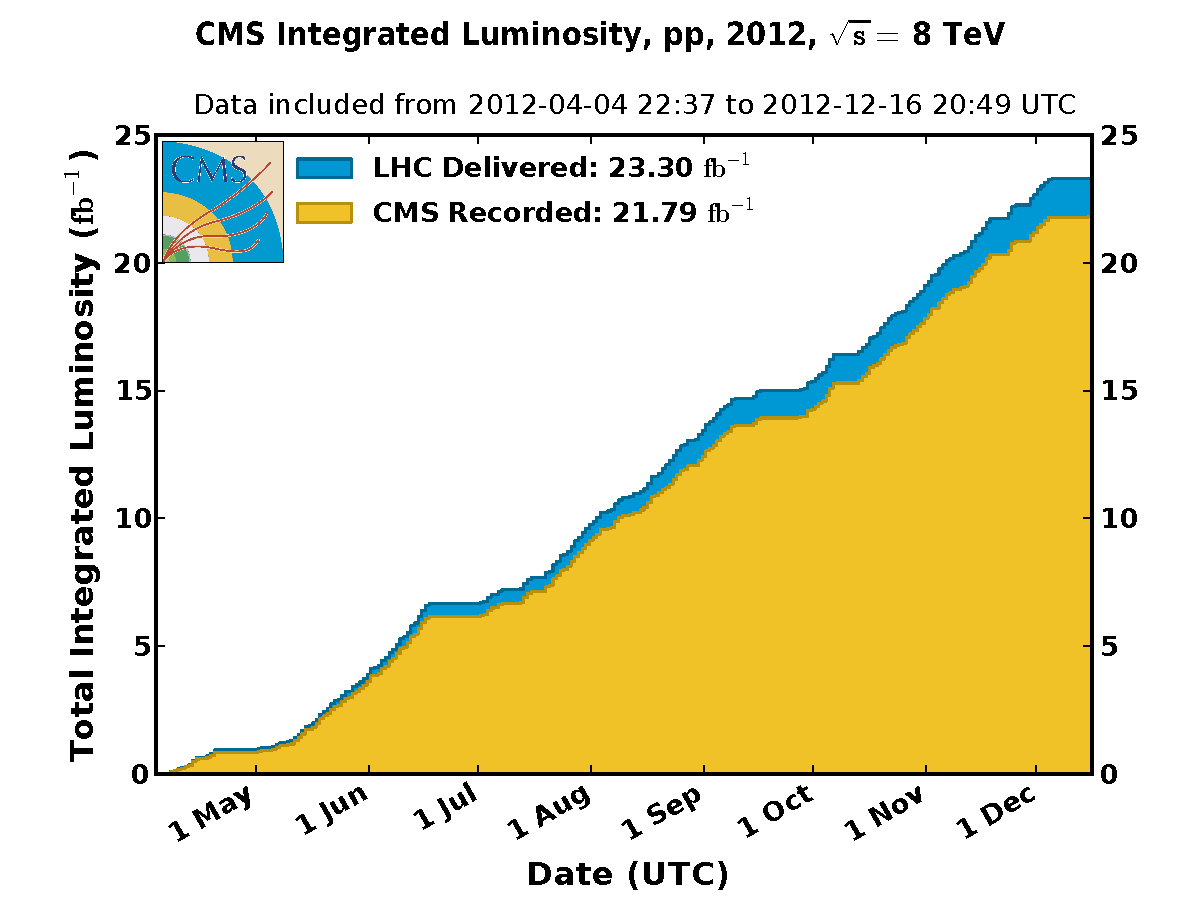
\includegraphics[width=\textwidth]{figures/2012_lumi.pdf}
    \caption{The integrate luminosity per day delivered and recorded by CMS in
        2012. The flat periods in May, July, and September correspond to the
        boundaries between the run eras.}
    \label{fig:2012_luminosity}
\end{figure}

The data collected by CMS are split into smaller datasets based on the physics
objects contained within the events. This allows analyses to use only one or
two datasets, instead of requiring them to deal with the entirety of the CMS
data (which is petabyte scale, and hence too large for most institutes to store
locally). The HLT sorts events into the various datasets based on the triggers
that the event fired. In this manner, an event can end up in multiple datasets
if it fired multiple triggers. This analysis uses the \SingleElectron dataset
which was collected with the HLT trigger \SingleElectronTrigger. These datasets
were reconstructed---converted from raw detector response into physics
objects---in January, 2013, in order to make use of the most recent
calibrations derived from the entire 2012 run. A summary of the datasets used
are listed in \TAB~\ref{table:datasets}.

\begin{table}[h]
\centering
\begin{center}
    \begin{tabular}{ | l | c | c |}
    \hline
    Dataset Name                          & Run Range      & Luminosity       \\ \hline
    /SingleElectron/Run2012A-22Jan2013-v1 & 190456--193621 & $889.362 \pbinv$ \\ \hline
    /SingleElectron/Run2012B-22Jan2013-v1 & 193833--196531 & $4.429 \fbinv$   \\ \hline
    /SingleElectron/Run2012C-22Jan2013-v1 & 198022--203742 & $7.152 \fbinv$   \\ \hline
    /SingleElectron/Run2012D-22Jan2013-v1 & 203777--208686 & $7.318 \fbinv$   \\ \hline
    \end{tabular}
\end{center}
\caption{
    The datasets used in this analysis. \TODO{Run range isn't useful, dates
    might be.}
}
\label{table:datasets}
\end{table}

Although there is a \DoubleElectron dataset which uses a trigger designed to
find Z bosons, this analysis uses the \SingleElectron dataset selected with the
\SingleElectronTrigger trigger. The primary motivation behind using this
trigger was to allow a direct comparison with a similar \phistar analysis being
performed by CMS which used \Ztomumu events selected with a single muon
trigger. The single electron trigger requires an electron with $\pt > 27$ which
passes Working Point 80 (\WPEighty), a set of selection requirements on lepton
isolation and shower shape designed to be 80\% efficient in selecting real
electrons. The requirements that make up \WPEighty are listed in
\TAB~\ref{table:wp80}. This trigger had the lowest \pt threshold of any single
electron trigger that was unprescaled run during 2012. To prescale a trigger
means to apply a rate reduction by randomly throwing out a certain fraction of
events in order to keep the total trigger rate manageable; as this trigger was
unprescaled, no events were discarded in this manner.

\begin{table}[h]
\centering
\begin{center}
    \begin{tabular}{ | c | c c |} \hline
        Value                      & EB     & EE     \\ \hline
        $|\eta| <$                 & 1.4791 & 2.65   \\
        $\pt >$                    & 27     & 27     \\
        $\sigmaietaieta <$         & 0.1    & 0.03   \\
        $\ECALISO / \et <$         & 0.15   & 0.1    \\
        $\HOverE <$                & 0.1    & 0.05   \\
        $\HCALISO / \et <$         & 0.1    & 0.1    \\
        Pixel Matching $\ge$       & 1      & 1      \\
        $|\ooeoop| <$              & 0.05   & 0.05   \\
        $|\Delta \eta| <$          & 0.007  & 0.007  \\
        $|\Delta \phi| <$          & 0.06   & 0.03   \\ \hline
    \end{tabular}
\end{center}
\caption{
    The selection requirements for the \SingleElectronTrigger trigger for
    electrons which end up in the barrel region or the endcap region of ECAL.
    The variables used are detailed in \SEC~\ref{sec:electron_variables}.
}
\label{table:wp80}
\end{table}

The events from the \SingleElectron sample are further filtered for quality. A
centrally produced list of good luminosity segments is used to select only
events in which no part of the detector was malfunctioning or disabled. After
accounting for detector dead time and beam quality, \GoodLumiNumber of
integrated luminosity are used for physics analysis.

\section{Object Selection}

\subsection{Electron Selection}
\label{ssec:electron_selection}

The requirements used to select electrons are chosen to be tighter than the
requirements used at the trigger level in order to make calculating the various
efficiencies easier. For an event to be considered it must have at least two
electrons that pass the acceptance requirements for \ExtendedElectrons: $\pt >
20 \GeV$ and $|\eta| < 2.4$. If three or more electrons pass this initial
requirement, only the two wit the highest \pt are considered. One of these two
electrons must be within $|\eta| < 2.1$ and it must also have $\pt > 30 \GeV$.

There are several centrally defined ``cut based identification'' requirements
used in electron selection at CMS. We use two of these, referred to as
\EGMEDIUM and \EGTIGHT, with \EGTIGHT having stricter requirements than
\EGMEDIUM. The exact definition of these requirements are given in
\TAB~\ref{table:eg_cuts}.

\begin{table}[h]
\centering
\begin{center}
    \begin{tabular}{ | c | c  c | c  c |} \hline
        \multirow{2}{*}{Variable}     & \multicolumn{2}{c |}{\EGTIGHT}    & \multicolumn{2}{c |}{\EGMEDIUM} \\
                                      & EB        & EE        & EB        & EE \\ \hline
        $\detain <$                   & 0.004     & 0.005     & 0.004     & 0.007 \\
        $\dphiin <$                   & 0.03      & 0.02      & 0.06      & 0.03 \\
        $\sigmaietaieta <$            & 0.01      & 0.03      & 0.01      & 0.03 \\
        $\HOverE <$                   & 0.12      & 0.10      & 0.12      & 0.10 \\
        $d_{0} <$                     & 0.02      & 0.03      & 0.02      & 0.02 \\
        $d_{z} <$                     & 0.1       & 0.1       & 0.1       & 0.1 \\
        $|\ooeoop| <$                 & 0.05      & 0.05      & 0.05      & 0.05 \\
        $\pvtx <$                     & $10^{-6}$ & $10^{-6}$ & $10^{-6}$ & $10^{-6}$ \\
        $\nmiss \le$                  & 0         & 0         & 1         & 1 \\
        $\PFISO / \pt^{\text{e}} <$   & 0.10      & 0.10      & 0.15      & 0.15 \\ \hline
    \end{tabular}
\end{center}
\caption{
    Identification and isolation requirements for \EGTIGHT and \EGMEDIUM
    requirements in the ECAL barrel (EB) and ECAL endcap (EE).
    The variables used are detailed in \SEC~\ref{sec:electron_variables}.
}
\label{table:eg_cuts}
\end{table}

A \CentralElectron in the event is required to pass \EGTIGHT and to be matched
to one of the electrons that passed \SingleElectronTrigger with $\Delta R <
0.3$. The other electron must pass \EGMEDIUM. If both electrons are
\CentralElectrons, then only one of them need pass \EGTIGHT, but this same
electron must also match the trigger; the other \CentralElectron need only pass
\EGMEDIUM.

No charge requirement is applied as even the same sign electron sample is
dominated by actual \Z decays as demonstrated by the large peak in the \mee
distribution.

The distributions of electron \pt and $\eta$ for the highest \pt electron and
the second highest \pt electron after all selection requirements are applied
are shown in \FIGS~\ref{fig:e_pt} and \ref{fig:e_eta}.

\begin{figure}[!htbp]
    \centering
    \begin{subfigure}[b]{0.65\textwidth}
        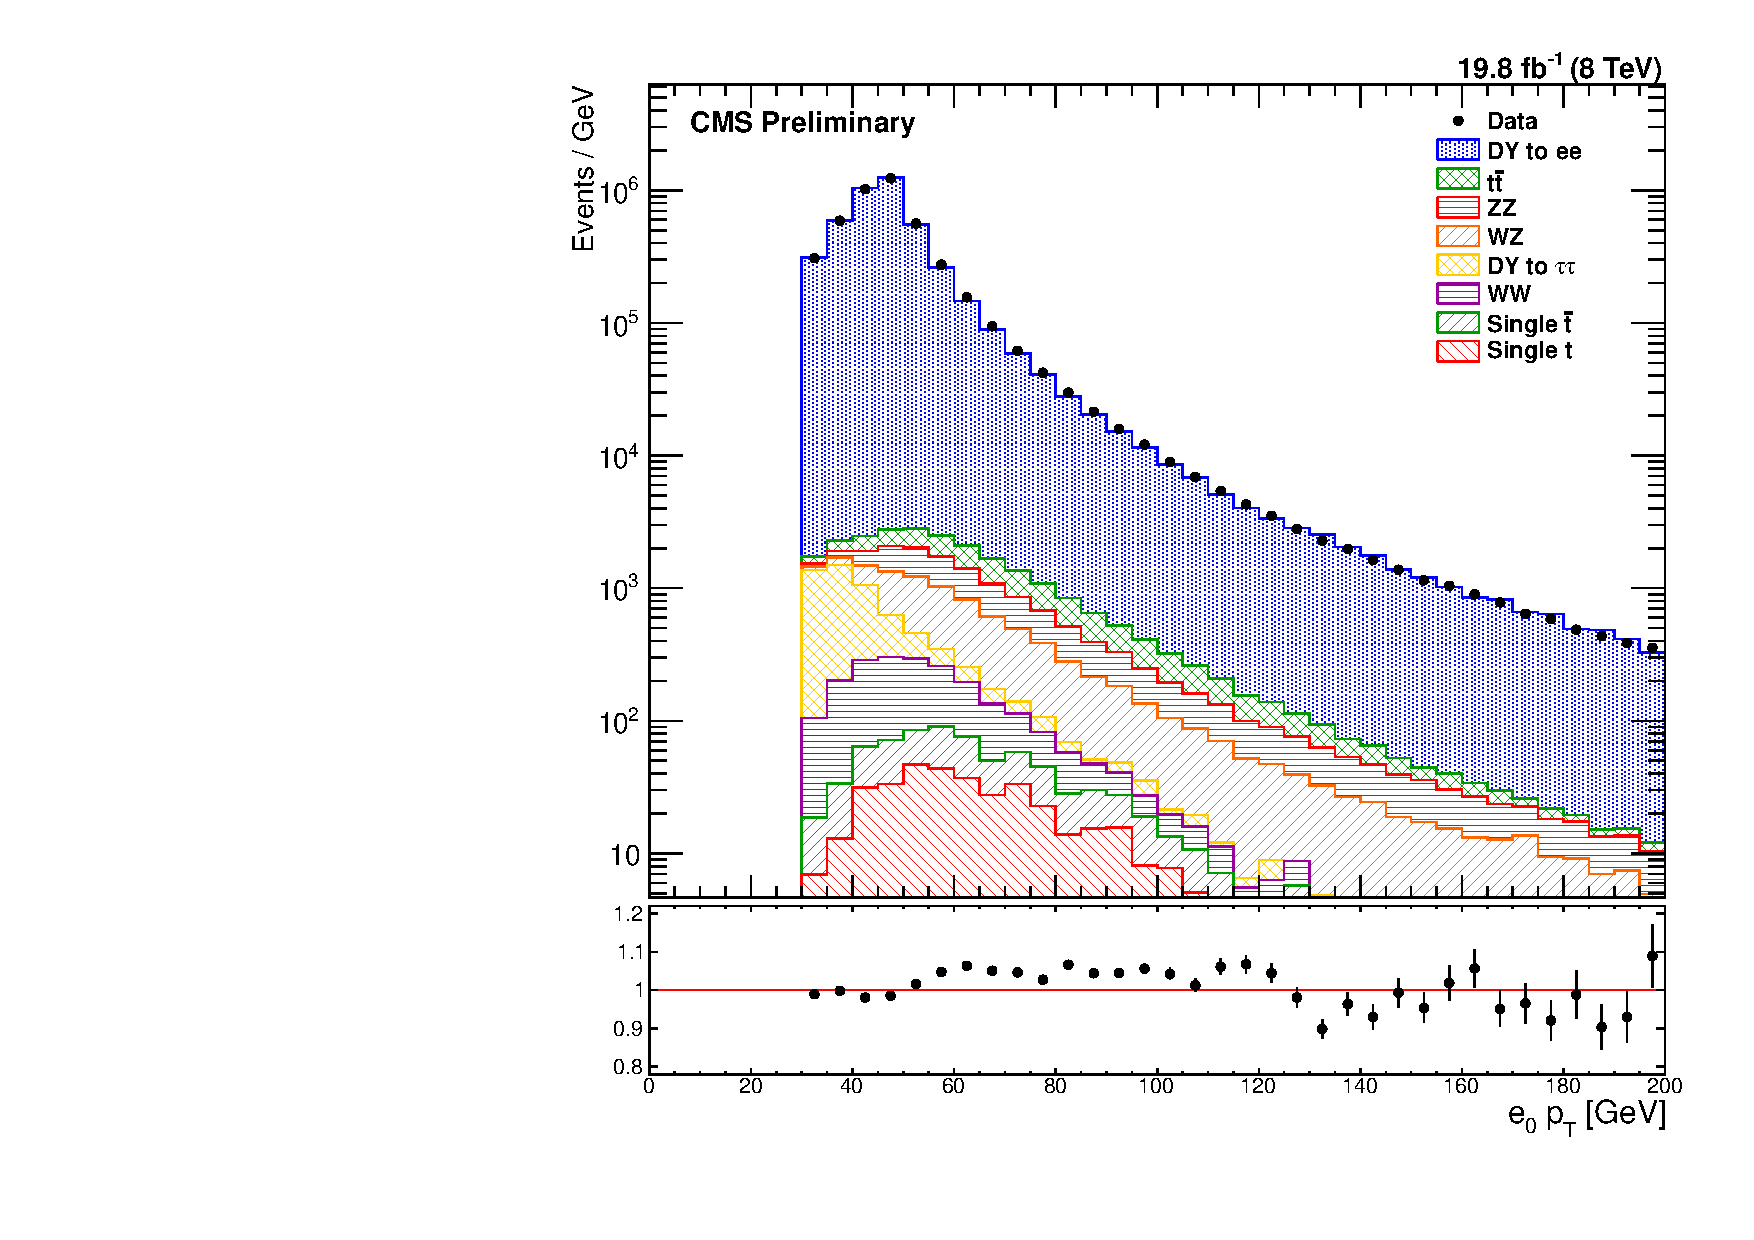
\includegraphics[width=\textwidth]{figures/e0_pt.pdf}
        \caption{}
        \label{fig:e_pt_high}
    \end{subfigure}
    \begin{subfigure}[b]{0.65\textwidth}
        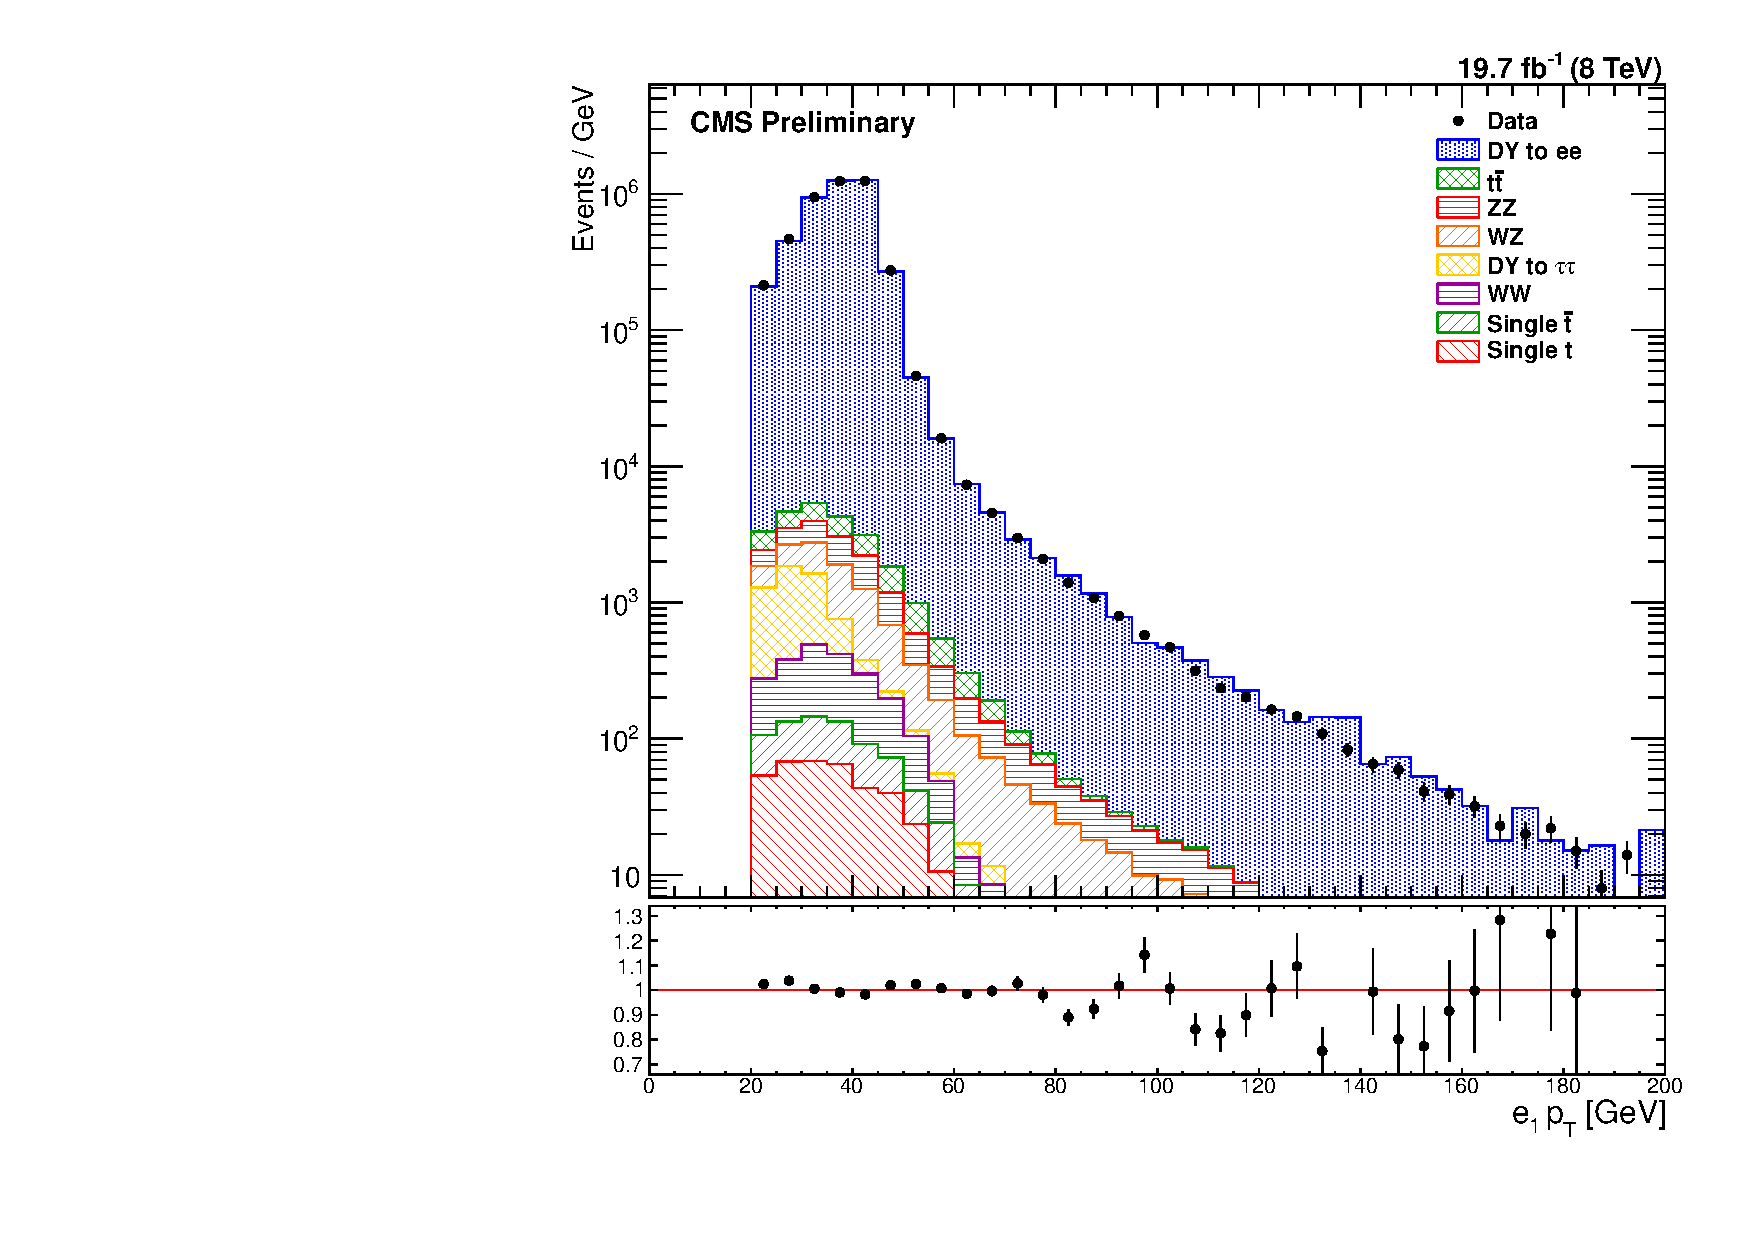
\includegraphics[width=\textwidth]{figures/e1_pt.pdf}
        \caption{}
        \label{fig:e_pt_low}
    \end{subfigure}
    \caption{
        The \pt distribution of the higher (top) and lower (bottom) \pt
        electrons in data (points) and MC (histograms) for events passing the
        full analysis selection.
    }
    \label{fig:e_pt}
\end{figure}

\begin{figure}[!htbp]
    \vspace*{\fill}
    \centering
    \begin{subfigure}[b]{0.65\textwidth}
        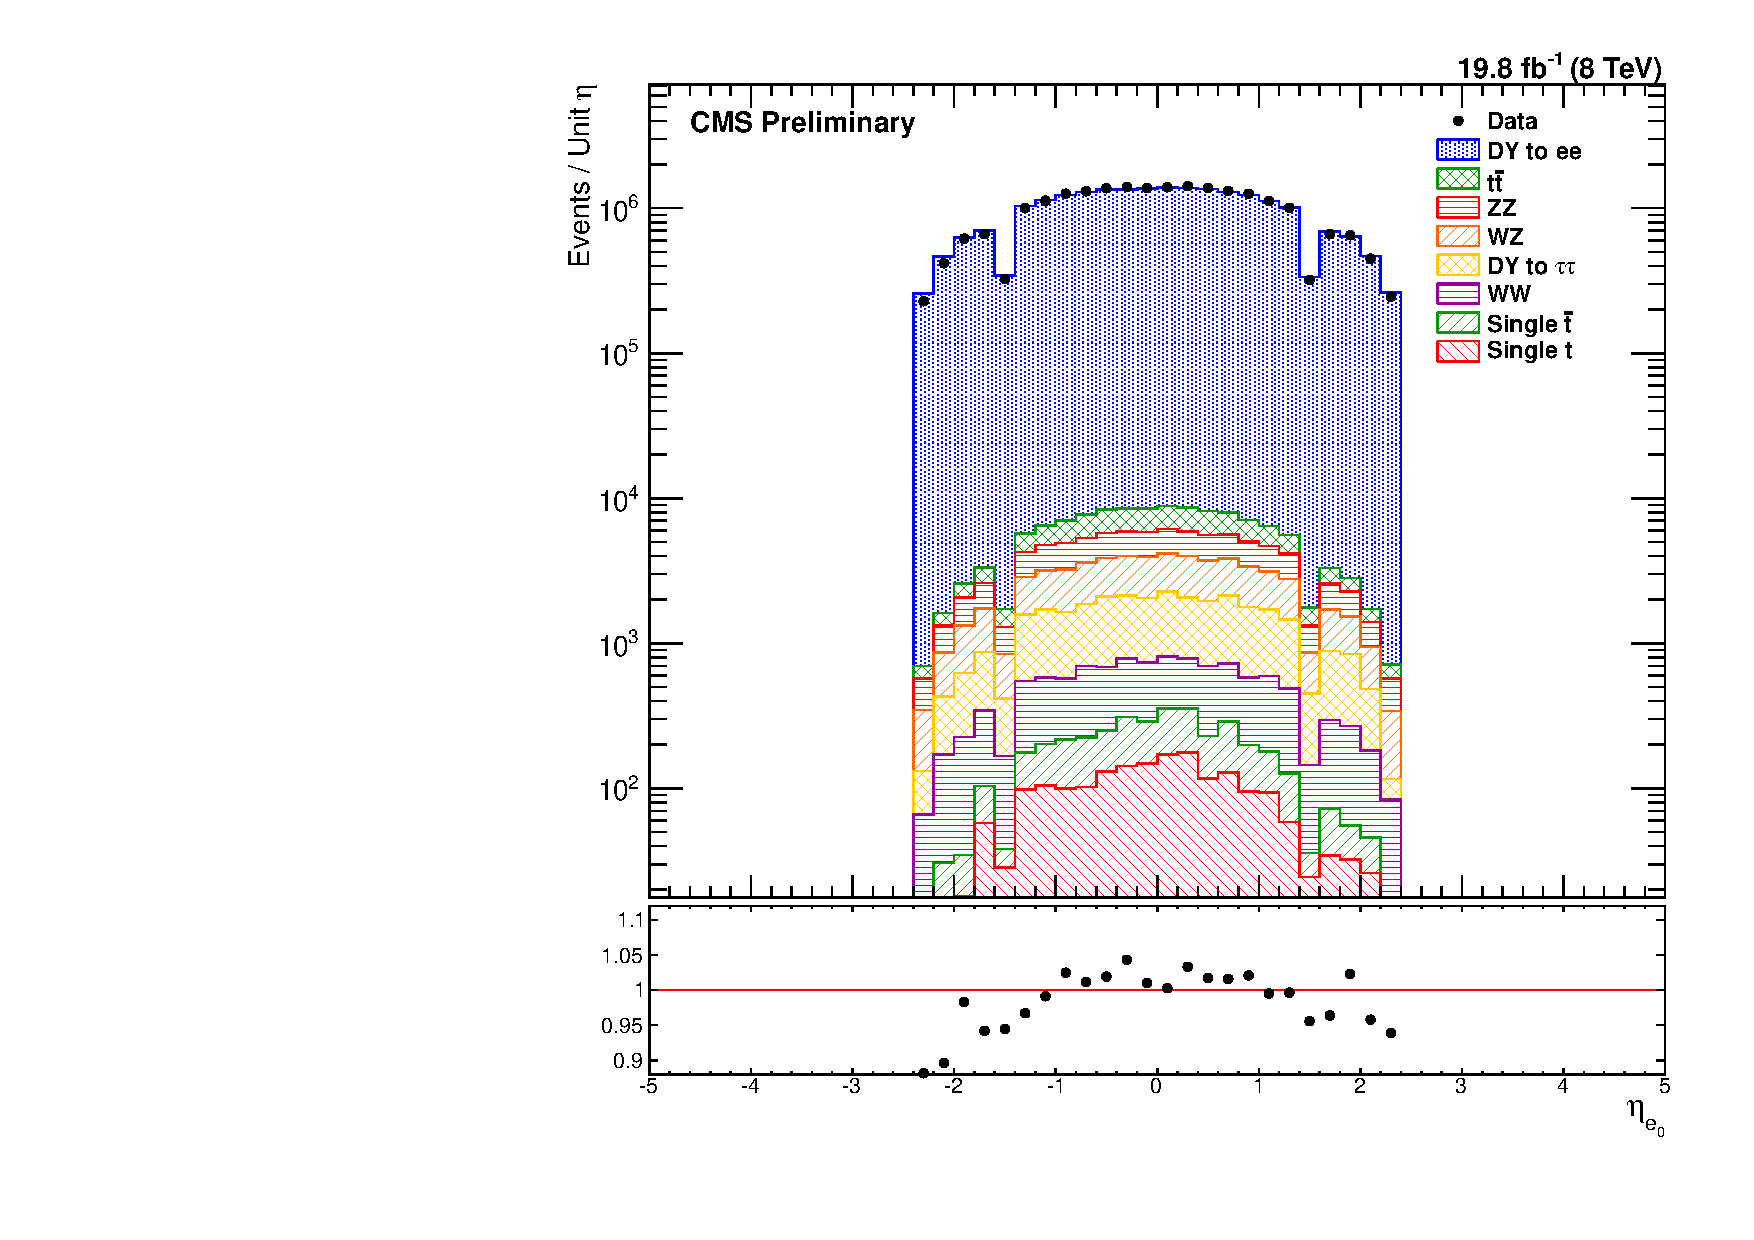
\includegraphics[width=\textwidth]{figures/e0_eta.pdf}
        \caption{}
        \label{fig:e_eta_high}
    \end{subfigure}
    \begin{subfigure}[b]{0.65\textwidth}
        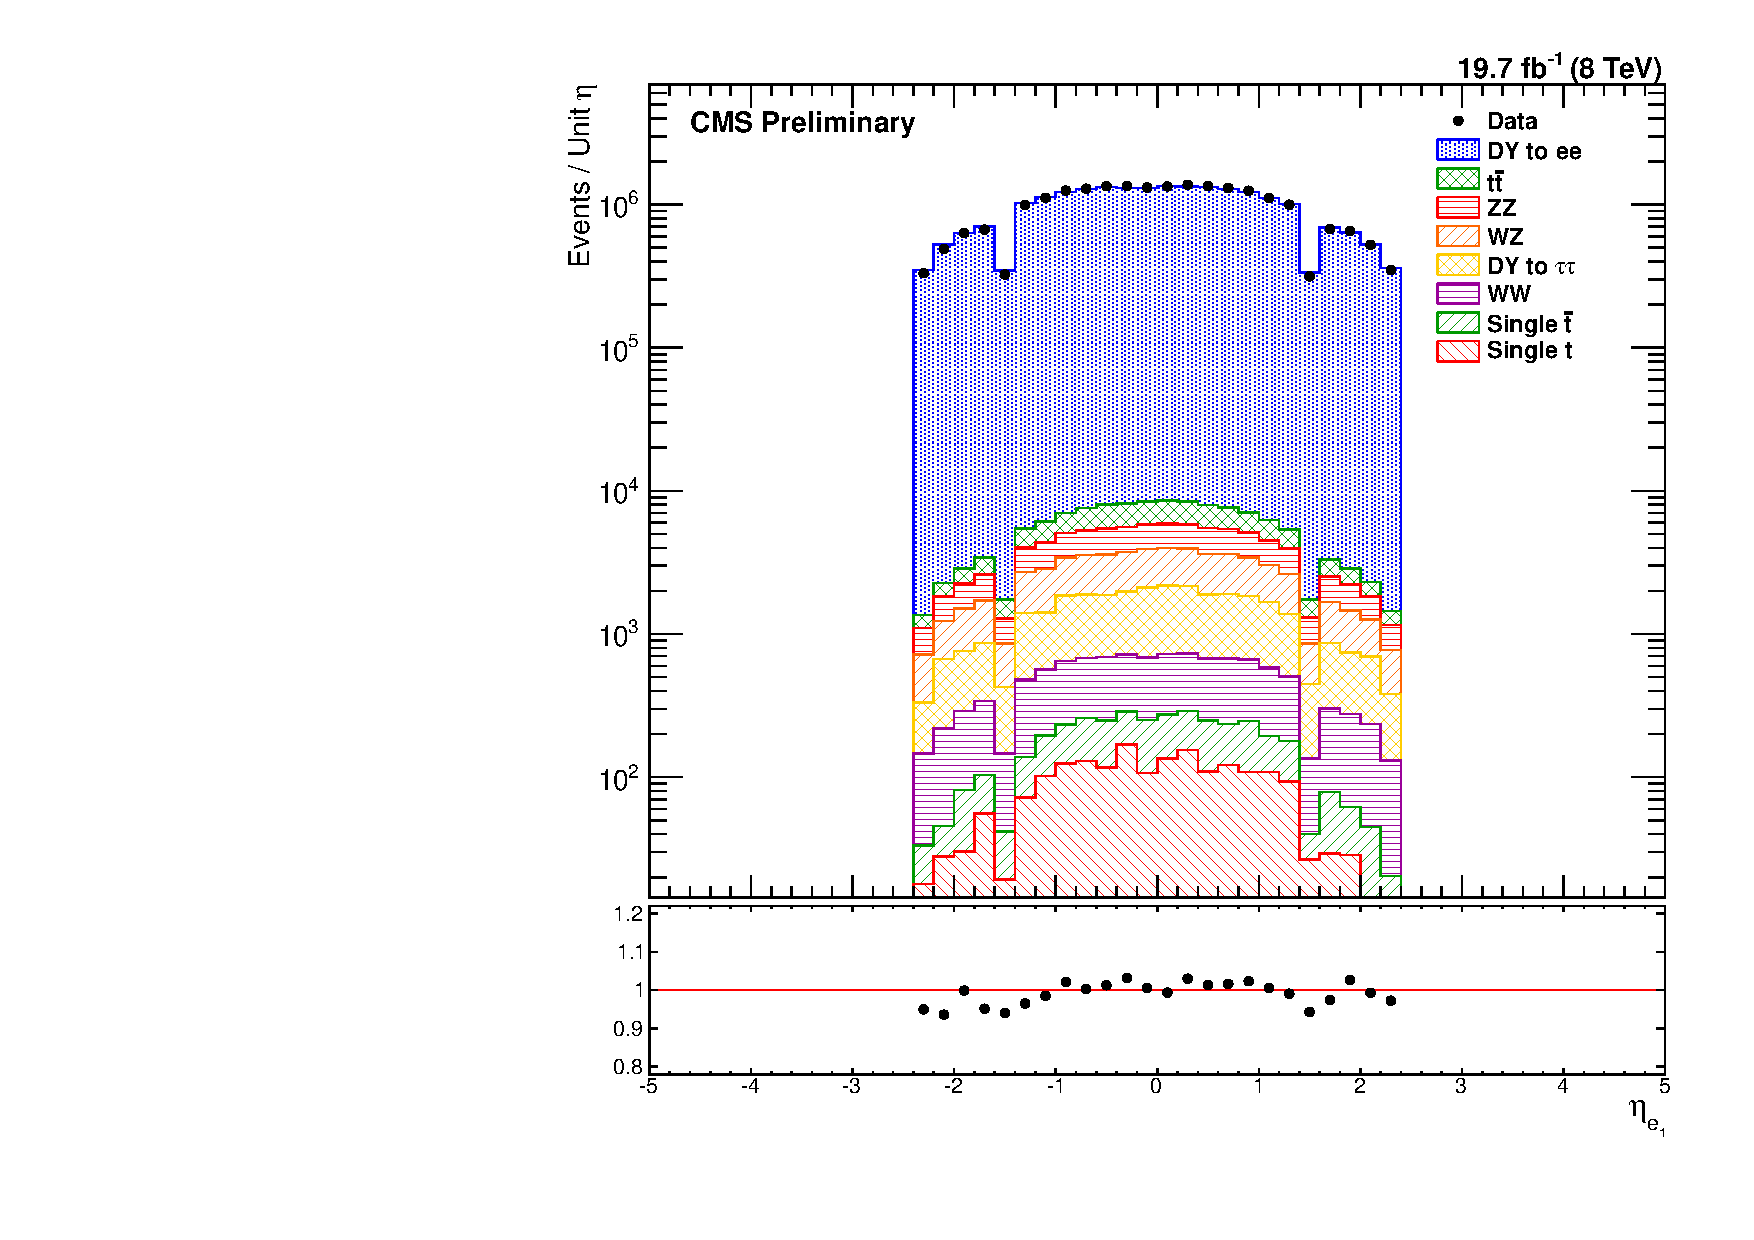
\includegraphics[width=\textwidth]{figures/e1_eta.pdf}
        \caption{}
        \label{fig:e_eta_low}
    \end{subfigure}
    \caption{
        The $\eta$ distribution of the higher (top) and lower (bottom) \pt
        electrons in data (points) and MC (histograms) for events passing the
        full analysis selection.
    }
    \label{fig:e_eta}
\end{figure}

\subsection{\Z Selection}

The \Z boson decays too quickly to leave any direct signal in the detector, so
it is reconstructed from its decay products: the two electrons whose selection
is described in \SEC~\ref{ssec:electron_selection}. In events where the two
electrons pass the selection, the \Z is constructed by taking the sum of the
electrons four-vectors. The resulting invariant mass of the \Z must be within
the region set by the acceptance (\MassRange).

The distributions of \mee, \Z \pt, and \Z \rapidity after these selection
requirements are applied are shown in \FIGS~\ref{fig:z_mass}, \ref{fig:z_pt},
and \ref{fig:z_rapidity}.

\begin{figure}[!htbp]
    \centering
    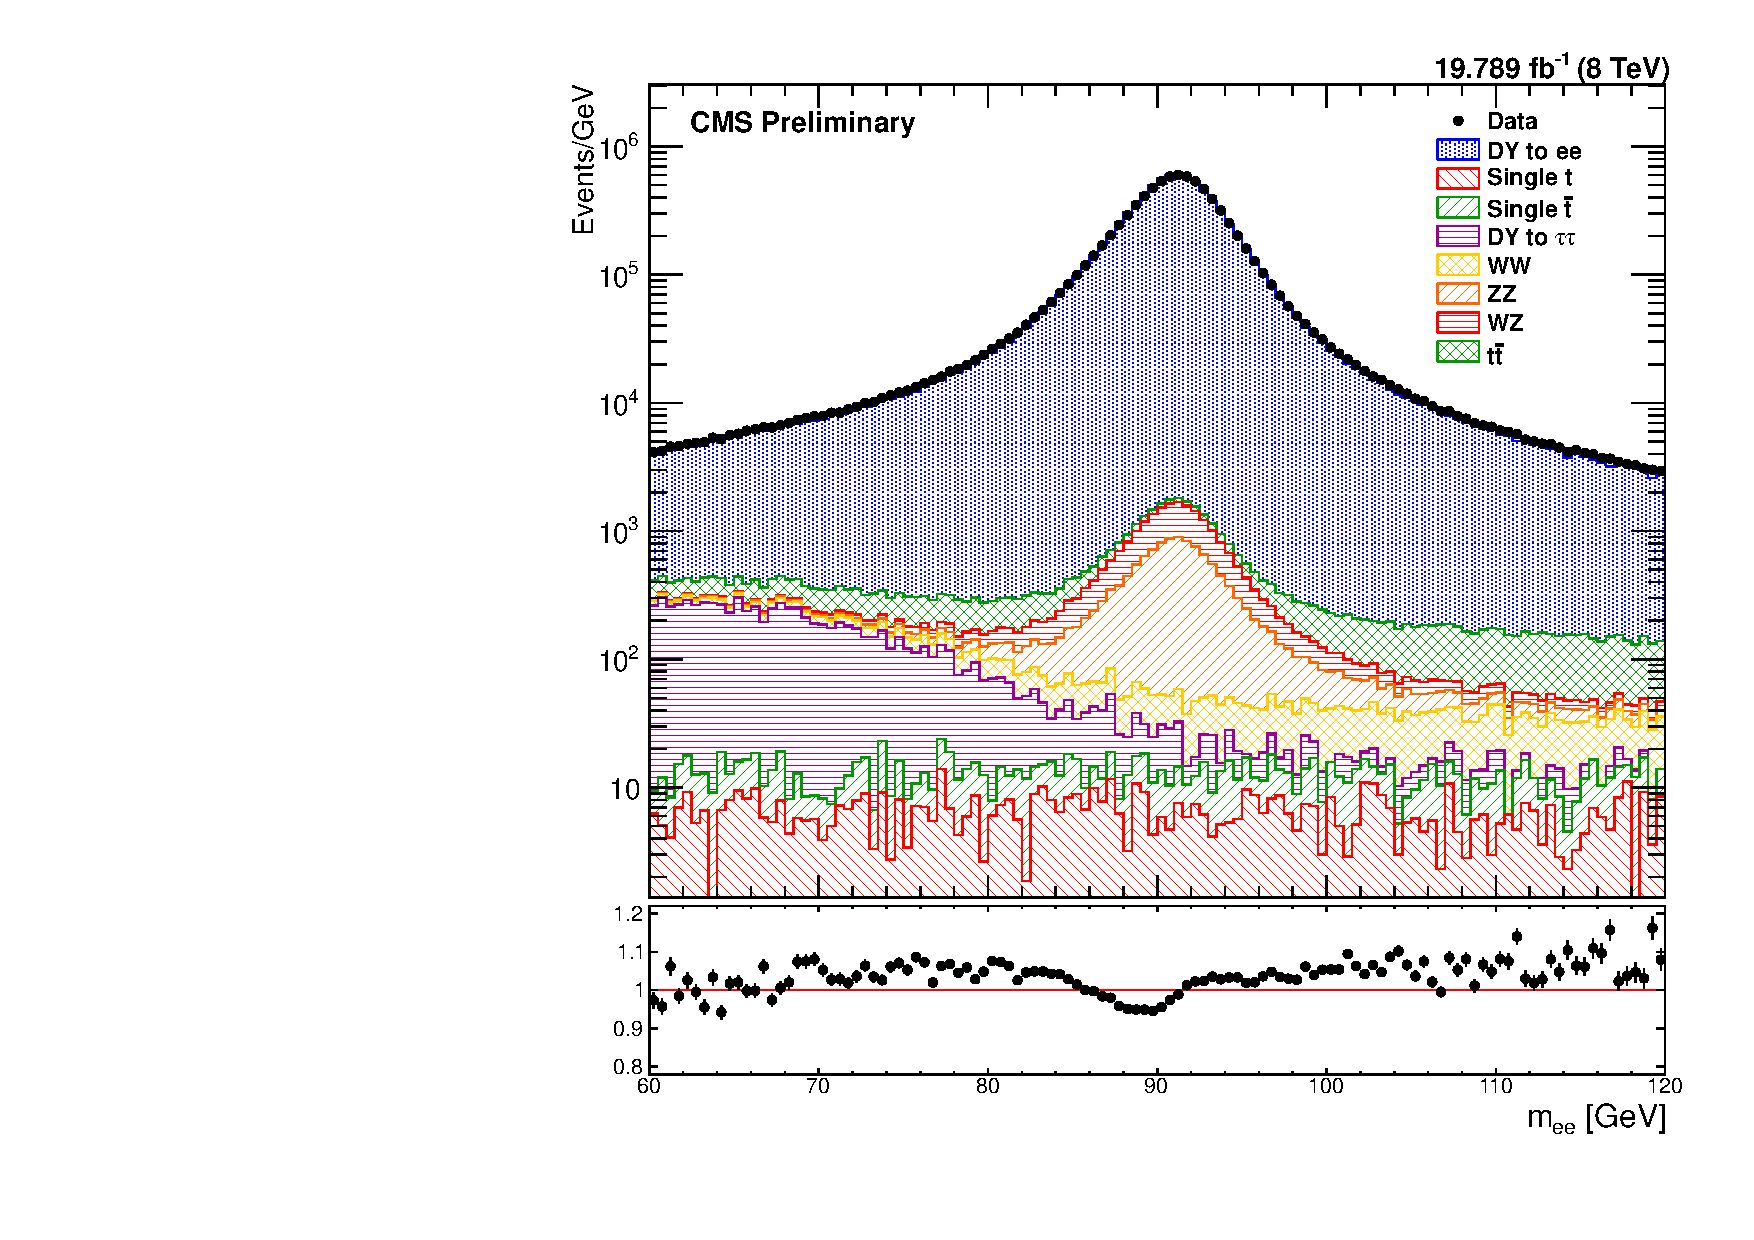
\includegraphics[width=\textwidth]{figures/z_mass_fine.pdf}
    \caption{
        The \mee distribution of all events passing the final selection in data
        (points) and MC (histograms).
    }
    \label{fig:z_mass}
\end{figure}

\begin{figure}[!htbp]
    \centering
    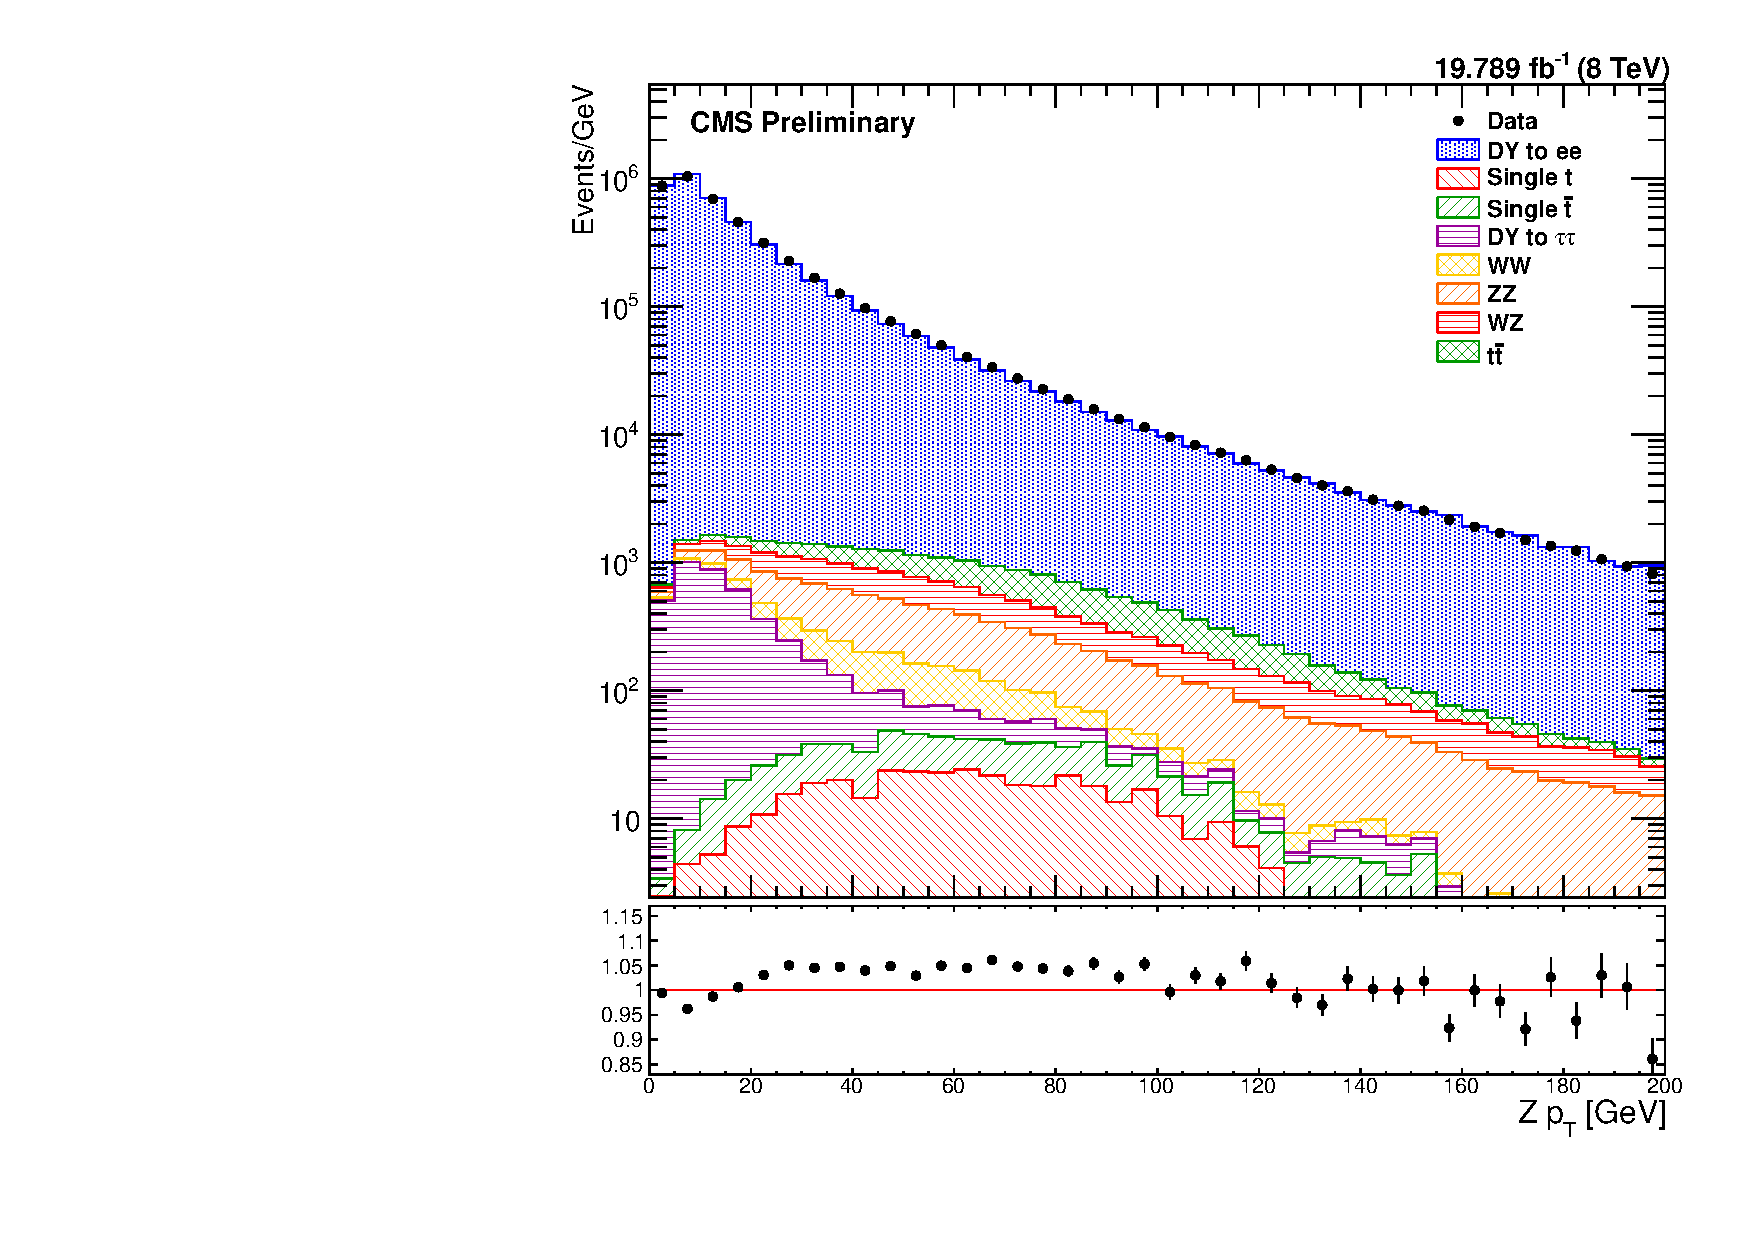
\includegraphics[width=\textwidth]{figures/z_pt.pdf}
    \caption{
        The $\pt$ distribution of \Z bosons for all events passing the final
        selection in data (points) and MC (histograms).
    }
    \label{fig:z_pt}
\end{figure}

\begin{figure}[!htbp]
    \centering
    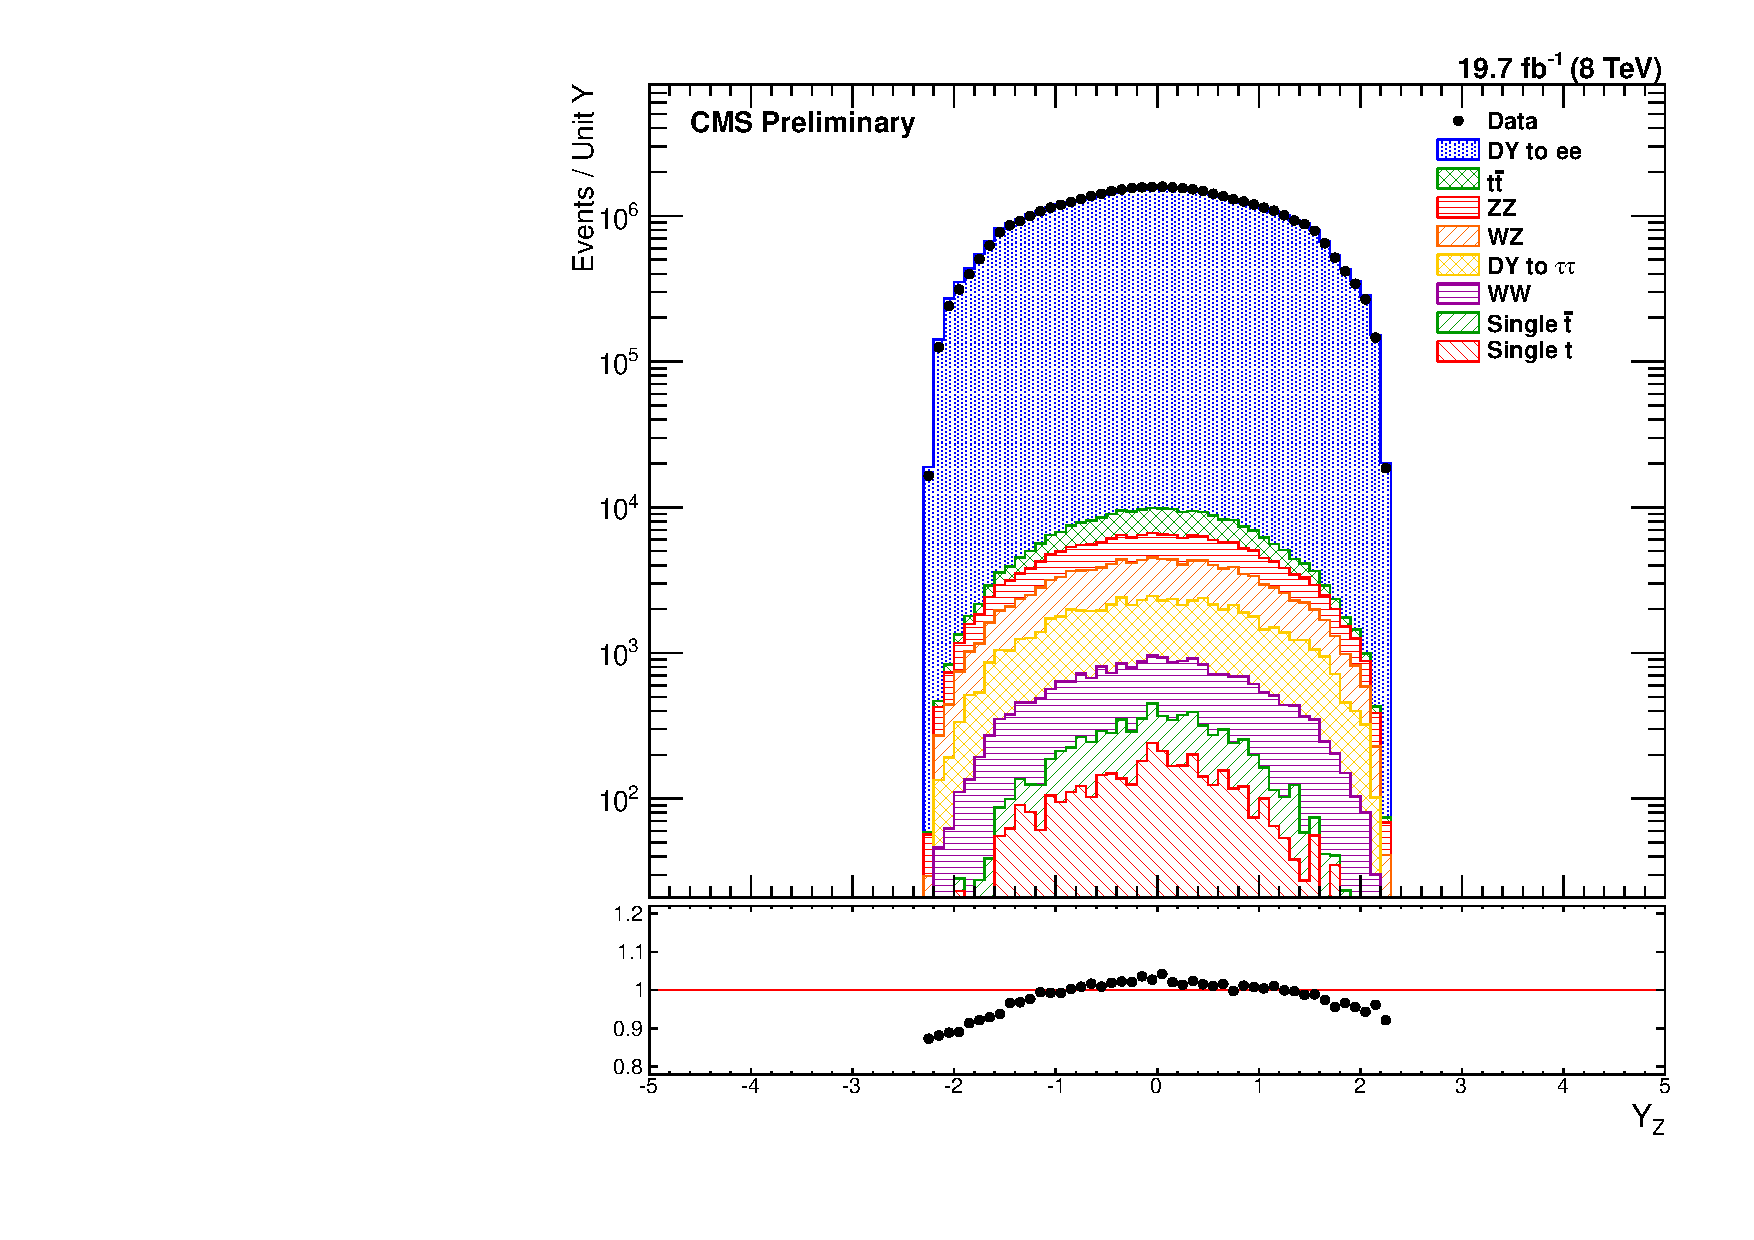
\includegraphics[width=\textwidth]{figures/z_rapidity.pdf}
    \caption{
        The $\rapidity$ distribution of \Z bosons for all events passing the
        final selection in data (points) and MC (histograms).
    }
    \label{fig:z_rapidity}
\end{figure}

\section{Background Estimation}

The distribution of background events is estimated using the MC samples
discussed in \SEC~\ref{ssec:monte_carlo}, with the \TODO{exception of QCD
related backgrounds, which are computed using data}. The various MC samples are
reweighed so that they have equivalent luminosity to the data. The MC datasets
also have various corrections applied which are discussed in
\SEC~\ref{sec:scale_factors}. These scale factors are applied as weights to
each MC event in order to make them better match the data.

After the reweighting, the selection requirements are applied to to the MC. The
number of events that survive the selection are taken as the number in our
data, and are subtracted off from the data events.

\begin{table}[h]
\centering
\begin{center}
    \begin{tabular}{ | l | r | r |}
    \hline
    Process           & of total & of background \\ \hline
    Signal: $\DYtoee$ &  99.53\% & N.A. \\
    \ttbar            &   0.14\% & 30.9\% \\
    $\Z\Z$            &   0.13\% & 27.2\% \\
    $\W\Z$            &   0.12\% & 25.9\% \\
    $\W\W$            &   0.03\% &  6.8\% \\
    $\DYtotautau$     &   0.03\% &  5.8\% \\
    $t\W + \tbar\W$   &   0.02\% &  3.4\% \\ \hline
    \end{tabular}
\end{center}
\caption{
    Data sample composition as a percentage of the total, as well as the
    backgrounds as a percentage of all background events.
    \TODO{Add QCD, double check these numbers are up-to-date.}
}
\label{table:bg_percentages}
\end{table}

Overall, the selection requirements discussed in the previous sections leave a
very pure sample of \Z boson events. \TODO{99.5\% of events are signal.} The dominant
backgrounds are the diboson backgrounds and \ttbar. We define \Z bosons
produced in association another weak boson as a background because of their
different production mechanism as opposed to single \Z boson events. The
fraction of events from each of the considered backgrounds is listed in
\TAB~\ref{table:bg_percentages}.

\TODO{Put \phistar plot with backgrounds.}

\subsection{\emu Control Samples}

Many of the backgrounds---specifically $\ttbar$, $\W\W$, $\DYtotautau$, and
$\ttbar$---produce leptons via independent decay chains. Therefore, the flavor
of the two leptons is not constrained to be the same. An electron--muon
(\emu) background dominated control sample is used to test how well the MC
reproduce the various backgrounds.

Events for the \emu sample are selected from data taken with the
\SingleMuonTrigger. This trigger required a single muon with $\pt > 24 \GeV$
and $|\eta| < 2.1$. Events selected from the dataset provided by this trigger
are required to have one muon with $\pt > 25 \GeV$ and $|\eta| < 2.1$ and one
electron with $\pt > 20 \GeV$ and $|\eta| < 2.4$. In order to further suppress
\Z decays, events are rejected if there is a third lepton of either flavor with
$\pt > 20 \GeV$ and $|\eta| < 2.4$. \TODO{\FIG~\ref{fig:emu_background_check}
shows a comparison of the MC and data in the control region. } Although no
deviations from \num{1} are seen in the ratio, the ratio is taken as a SF to
correct the previously listed backgrounds in each bin.

\begin{figure}[!htbp]
    \centering
    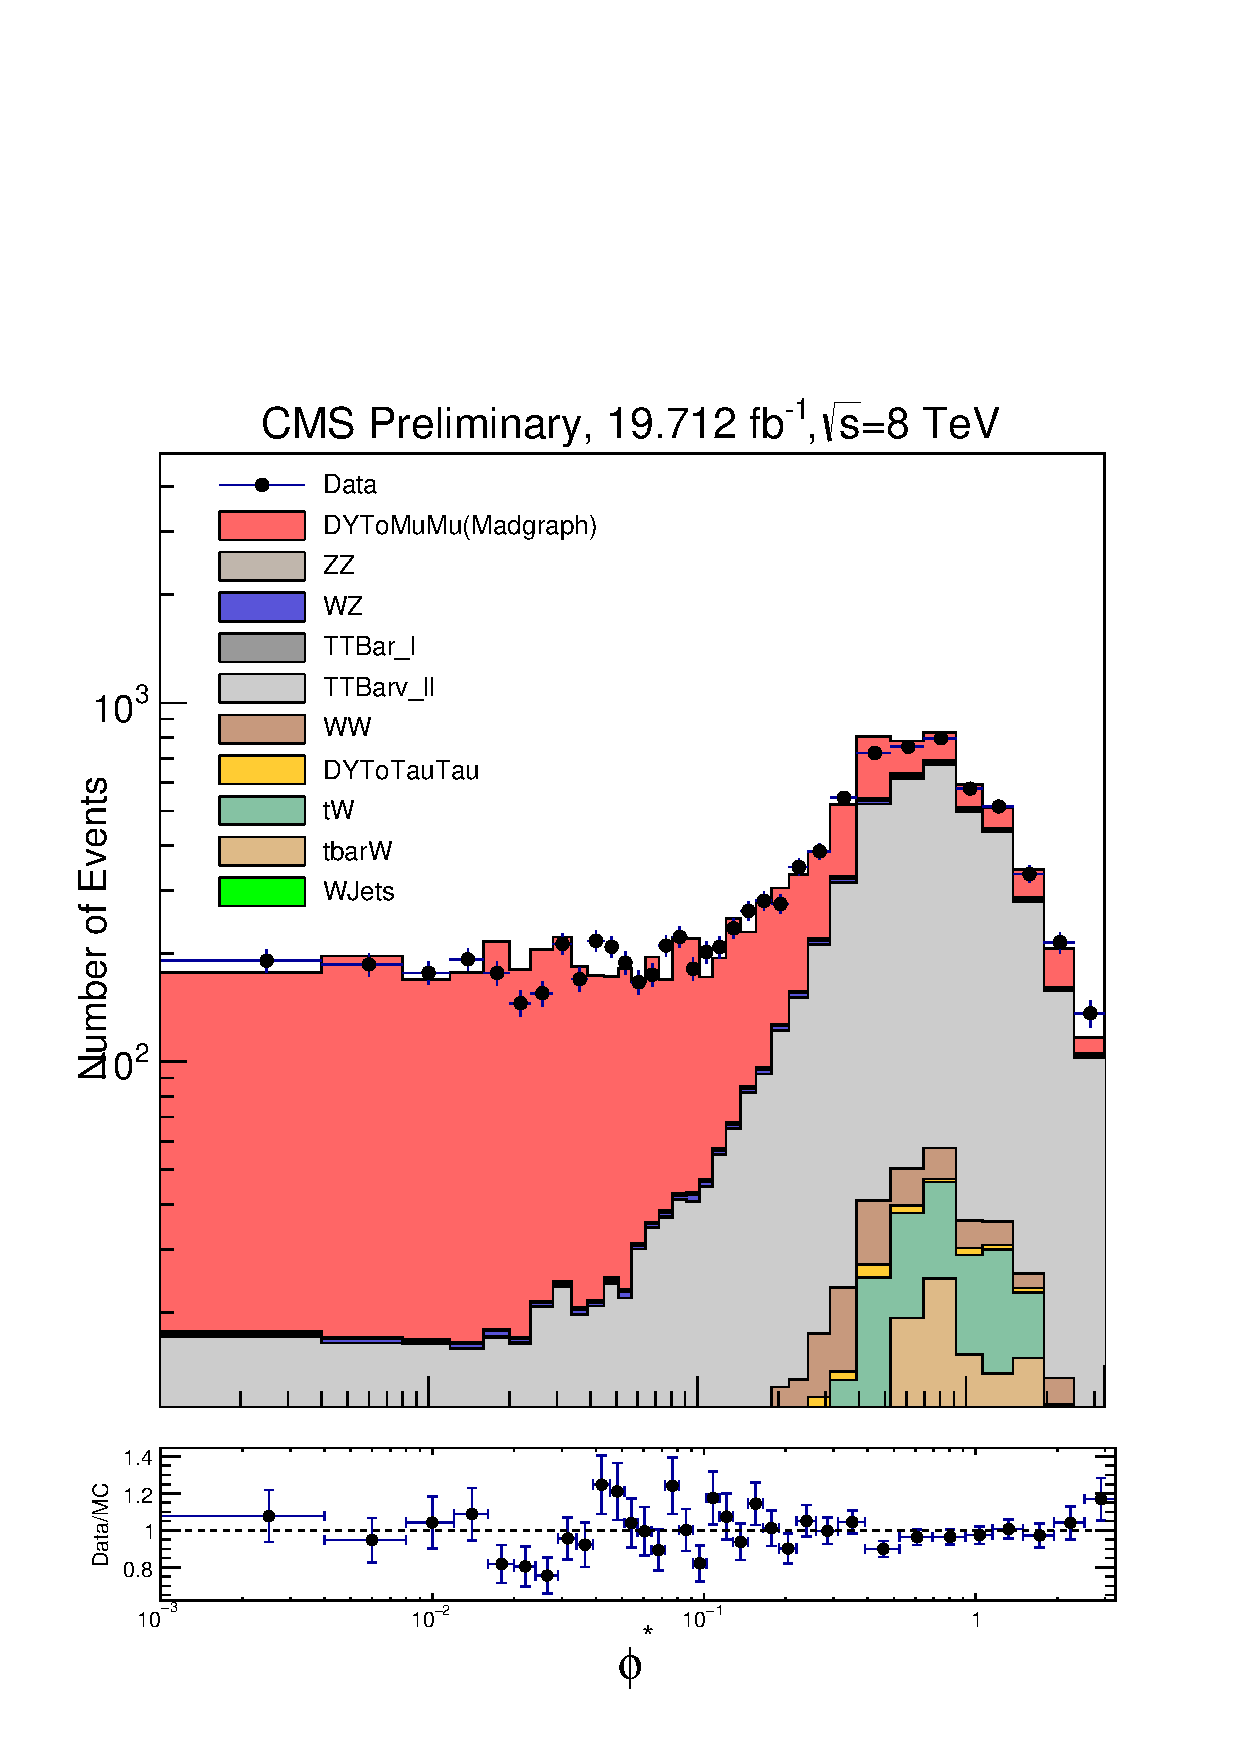
\includegraphics[width=\textwidth]{figures/phistar_emu.pdf}
    \caption{
        The \phistar distribution of events from the \emu control sample. The
        data (points) match the MC (histograms) expectation well. The ratio,
        shown in the bottom plot, is taken as a SF and used to correct the
        backgrounds in each bin.
    }
    \label{fig:emu_background_check}
\end{figure}

\TODO{Does this go in the uncertainty section? "This method could not be used
    to calibrate the $\Z\Z$ and $\Z\W$ background MC samples as they contain
    actual \Z bosons. Instead a 20\% uncertainty is taken on their theoretical
    cross-section."}

\subsection{QCD Background Estimation}

The centrally produced QCD MC does not have enough events to make an accurate
estimation of the QCD background in this analysis so instead a data driven
method is employed. The same requirements as discussed in
\SEC~\ref{ssec:electron_selection} are applied to both the data and the MC
samples with the additional requirement that both electrons must have the same
sign. This additional selection requirement removes most of the signal while
removing only half of the expected QCD background. This is because the QCD
processes are independent and hence there is no correlation between the charge
of the two leptons.

The data and MC are divided into subsamples with each subsample corresponding
to a bin in the \phistar distribution. The \mee distribution of the events in
each data subsample is fit with a combination of an MC template and an analytic
QCD background function.

The MC templates used in the fit are created by reweighting each MC sample to
have the same luminosity as the data. These MC samples are then added together to
form a combined MC sample that includes both the MC \MADGRAPH signal sample and
the various background MC samples. The shape of this combined sample in each
\phistar bin is taken as a template when fitting the corresponding bin in data.

The analytic QCD background function, $\BGFunc$, is the same function used by
Haupt to model the QCD background in his \Ztoee shape measurement
\cite{haupt_2011}. It is composed of a falling exponential---which fits the
general shape of the QCD distribution---multiplied by a complementary error
function---which cuts off the exponential at low mass. The exact form of this
function is given by \EQ~\ref{eq:haupt_function}. The sum of the template and
the background function is given by \EQ~\ref{eq:qcd_fit_function}.

The background due to QCD in each \phistar bin is taken to be the integral of
the analytic background component from \MassRange. \TODO{Two example fits are
shown in \FIG~\ref{fig:qcd_example_fits}. All of the fits are shown in
\APP~\ref{app:qcd_fits}.}

\begin{equation}\label{eq:haupt_function}
    \BGFuncArgs = e^{- \gamma x} \erfc \left( \frac{\varepsilon - x}{\delta} \right)
\end{equation}

\begin{equation}\label{eq:qcd_fit_function}
    \alpha \, \MCTemplate + \beta \, \BGFuncArgs
\end{equation}

\TODO{\label{fig:same_sign_z_peak}}
\TODO{Example fits, appendix of all fits. \label{fig:qcd_example_fits}}
